% ============================================================================
% BABBAGE ANALYTICAL ENGINE - PHASE 2: BUILDOUT AND HARDWARE CONSTRUCTION
% PART 2: BSD INTEGRATION, ROADMAP, BUDGET, RISK, EXTENSIONS, CONCLUSION
% ============================================================================

\documentclass[11pt,oneside,openany]{book}

\usepackage[margin=1in]{geometry}
\usepackage{titlesec}
\usepackage{tikz}
\usepackage{pgfplots}
\usepackage{pgfplotstable}
\usepackage{booktabs}
\usepackage{hyperref}
\usepackage{listings}
\usepackage{xcolor}
\usepackage{amsmath}
\usepackage{amssymb}
\usepackage{setspace}

\pgfplotsset{compat=1.18}
\usetikzlibrary{shapes,arrows,positioning,calc}
\onehalfspacing

\definecolor{darkblue}{RGB}{25,55,109}
\definecolor{lightblue}{RGB}{173,216,230}
\definecolor{darkgreen}{RGB}{34,139,34}
\definecolor{lightgreen}{RGB}{144,238,144}
\definecolor{darkred}{RGB}{178,34,34}
\definecolor{lightyellow}{RGB}{255,255,200}

\titleformat{\chapter}{\Large\bfseries\color{darkblue}}{\thechapter.}{1em}{}
\titleformat{\section}{\large\bfseries\color{darkgreen}}{\thesection.}{1em}{}

\setcounter{chapter}{5}  % Continue from chapter 6

\title{\textbf{BABBAGE ANALYTICAL ENGINE - PHASE 2: PART 2}}
\author{Infrastructure Strategy Continuation}
\date{October 31, 2025}

\begin{document}

\chapter{BSD Integration: Device Driver and Kernel Interface}

\section{Architecture Overview: Two Integration Approaches}

\subsection{Option A: Device Driver Model (Recommended)}

Device driver approach:
\begin{itemize}
  \item Create character device \texttt{/dev/babbage}
  \item Use ioctl() system calls for operations
  \item Standard Unix device semantics (open, close, ioctl, read, write)
  \item Compatible across 2.11BSD, DiscoBSD, Linux
\end{itemize}

\begin{table}[h!]
\centering
\small
\begin{tabular}{llr}
\toprule
\textbf{ioctl Command} & \textbf{Purpose} & \textbf{Latency} \\
\midrule
\rowcolor{lightblue}
BABBAGE\_IOC\_LOAD & Load program to device & < 1 ms \\
\rowcolor{lightblue}
BABBAGE\_IOC\_RUN & Execute N steps & 1-100 ms \\
\rowcolor{lightgreen}
BABBAGE\_IOC\_STATUS & Get engine state & < 1 ms \\
\rowcolor{lightyellow}
BABBAGE\_IOC\_RESET & Reset to initial state & < 1 ms \\
\rowcolor{lightyellow}
BABBAGE\_IOC\_STEP & Single-step execution & 1-10 ms \\
\bottomrule
\end{tabular}
\caption{Device driver ioctl operations for Babbage engine control.}
\label{tab:ioctl_operations}
\end{table}

\subsection{Option B: System Call Interface}

System call approach:
\begin{itemize}
  \item Direct kernel interface: babbage\_load(), babbage\_run(), babbage\_status(), babbage\_reset()
  \item Lower overhead than ioctl()
  \item Requires kernel source modification
  \item Not portable across kernels (platform-specific)
\end{itemize}

\section{Device Driver Implementation Details}

\subsection{Kernel Module Structure}

\begin{figure}[h!]
\centering
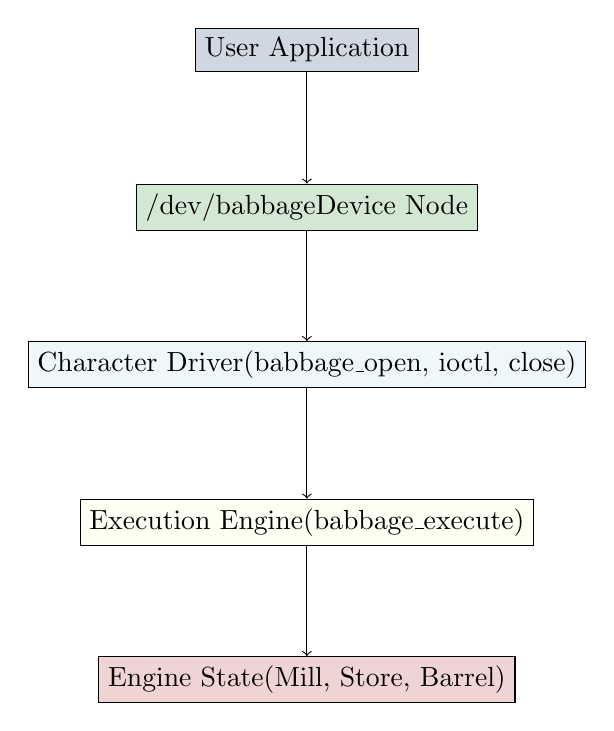
\begin{tikzpicture}[node distance=2cm]
  
  \node[rectangle,draw,fill=darkblue!20] (app) {User Application};
  \node[rectangle,draw,fill=darkgreen!20,below of=app] (devfs) {/dev/babbage\\Device Node};
  \node[rectangle,draw,fill=lightblue!20,below of=devfs] (char_drv) {Character Driver\\(babbage\_open, ioctl, close)};
  \node[rectangle,draw,fill=lightyellow!20,below of=char_drv] (exec_eng) {Execution Engine\\(babbage\_execute)};
  \node[rectangle,draw,fill=darkred!20,below of=exec_eng] (state) {Engine State\\(Mill, Store, Barrel)};
  
  \draw[->] (app) -- (devfs);
  \draw[->] (devfs) -- (char_drv);
  \draw[->] (char_drv) -- (exec_eng);
  \draw[->] (exec_eng) -- (state);
  
\end{tikzpicture}
\caption{Device driver architecture: layers from user application to engine state.}
\label{fig:driver_arch}
\end{figure}

\subsection{Babbage State Structure}

\begin{lstlisting}[language=C]
struct babbage_state {
    u_int32_t mill[5];              /* Accumulator digits 0-49 */
    u_int32_t ingress;              /* Input register */
    u_int32_t egress;               /* Output register */
    u_int32_t store[2000];          /* Memory columns 0-1999 */
    u_int16_t barrel_pos;           /* Barrel position (0-149) */
    u_int16_t pc;                   /* Program counter */
    u_int8_t  status;               /* Status: READY, RUNNING, ERROR */
    u_int8_t  carry;                /* Carry flag */
    u_int64_t cycles;               /* Total cycles executed */
    u_int32_t instructions;         /* Instructions executed */
};

struct babbage_softc {
    struct babbage_state state;
    int unit;
    int flags;
    u_char *program;
    int program_length;
};
\end{lstlisting}

\section{DiscoBSD 2.5 Integration Path}

\subsection{Target Platform: STM32F4 Discovery}

\begin{table}[h!]
\centering
\small
\begin{tabular}{llr}
\toprule
\textbf{Resource} & \textbf{Capacity} & \textbf{Babbage Need} \\
\midrule
\rowcolor{lightblue}
Flash (code) & 1 MB & 250 KB (kernel) + 50 KB (module) \\
\rowcolor{lightgreen}
SRAM (data) & 192 KB & 110 KB (Store + state) + 50 KB (buffers) \\
\rowcolor{lightyellow}
Speed & 168 MHz & Sufficient for emulation \\
\bottomrule
\end{tabular}
\caption{DiscoBSD 2.5 (STM32F4) resource allocation for Babbage kernel module.}
\label{tab:discobsd_resources}
\end{table}

\subsection{Memory Layout}

\begin{figure}[h!]
\centering
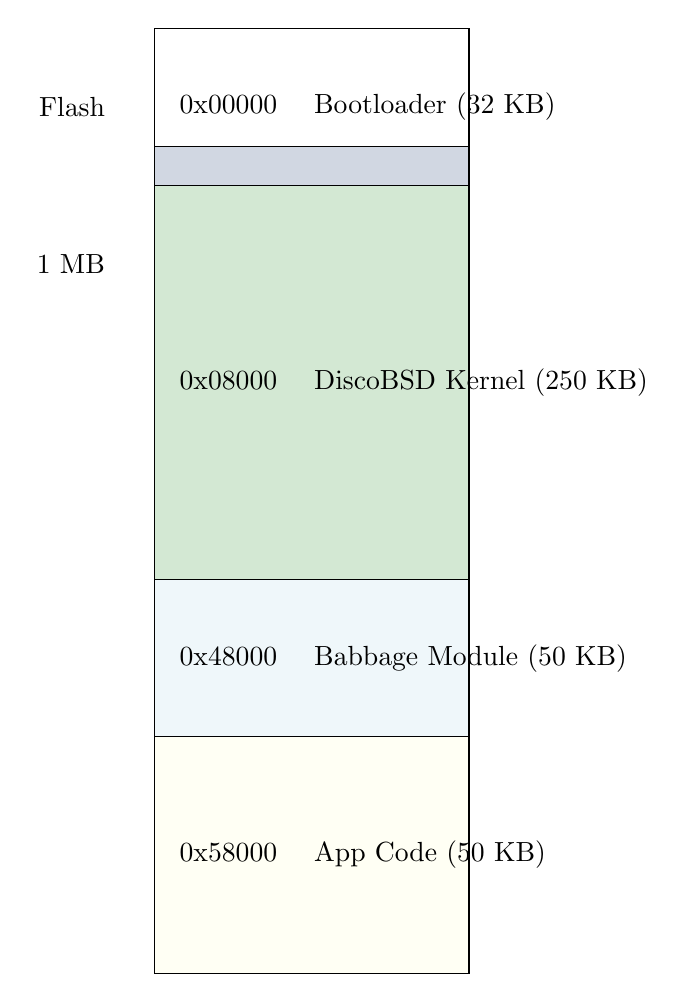
\begin{tikzpicture}
  % Memory regions
  \draw (0,0) rectangle (4,12);
  \node[anchor=west] at (0.2,11) {0x00000 \quad Bootloader (32 KB)};
  \draw[fill=darkblue!20] (0,10) rectangle (4,10.5);
  
  \draw[fill=darkgreen!20] (0,5) rectangle (4,10);
  \node[anchor=west] at (0.2,7.5) {0x08000 \quad DiscoBSD Kernel (250 KB)};
  
  \draw[fill=lightblue!20] (0,3) rectangle (4,5);
  \node[anchor=west] at (0.2,4) {0x48000 \quad Babbage Module (50 KB)};
  
  \draw[fill=lightyellow!20] (0,0) rectangle (4,3);
  \node[anchor=west] at (0.2,1.5) {0x58000 \quad App Code (50 KB)};
  
  % Labels
  \node[left] at (-0.5,11) {Flash};
  \node[left] at (-0.5,9) {1 MB};
\end{tikzpicture}
\caption{STM32F4 Flash memory layout: DiscoBSD kernel + Babbage module + app.}
\label{fig:memory_layout}
\end{figure}

\section{Cross-Platform Compatibility}

\begin{table}[h!]
\centering
\small
\begin{tabular}{lllr}
\toprule
\textbf{Platform} & \textbf{DiscoBSD} & \textbf{Implementation} & \textbf{Status} \\
\midrule
\rowcolor{lightblue}
STM32F4 (Cortex-M4) & 2.5 & Device driver & Recommended \\
\rowcolor{lightblue}
PIC32 & 2.5 & Device driver & Alternative \\
\rowcolor{lightgreen}
Raspberry Pi & 2.11BSD port & LKM or system call & Phase 3 \\
\rowcolor{lightyellow}
x86-64 (Linux) & N/A & Loadable kernel module & Phase 3 \\
\bottomrule
\end{tabular}
\caption{Cross-platform integration matrix: DiscoBSD 2.5 is primary target.}
\label{tab:platform_matrix}
\end{table}

% ============================================================================
% CHAPTER 7: INTEGRATION ROADMAP
% ============================================================================

\chapter{Integration Roadmap: Phased Timeline}

\section{Overall Schedule}

The Babbage Phase 2 project involves four parallel work streams:

\begin{figure}[h!]
\centering
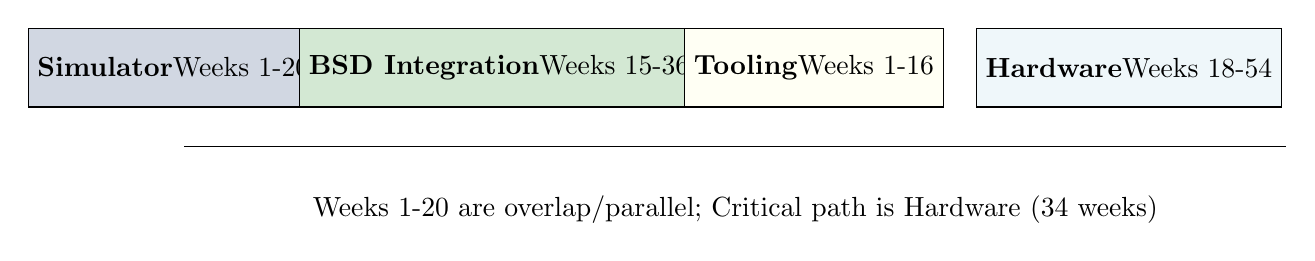
\begin{tikzpicture}[node distance=2cm]
  
  \node[rectangle,draw,fill=darkblue!20,minimum width=3cm,minimum height=1cm] (sim) at (0,4) {
    \textbf{Simulator}\\
    Weeks 1-20+
  };
  
  \node[rectangle,draw,fill=darkgreen!20,minimum width=3cm,minimum height=1cm] (bsd) at (4,4) {
    \textbf{BSD Integration}\\
    Weeks 15-36
  };
  
  \node[rectangle,draw,fill=lightyellow!20,minimum width=3cm,minimum height=1cm] (tool) at (8,4) {
    \textbf{Tooling}\\
    Weeks 1-16
  };
  
  \node[rectangle,draw,fill=lightblue!20,minimum width=3cm,minimum height=1cm] (hw) at (12,4) {
    \textbf{Hardware}\\
    Weeks 18-54
  };
  
  \draw (0,3) -- (14,3);
  \node[below] at (7,2.5) {Weeks 1-20 are overlap/parallel; Critical path is Hardware (34 weeks)};
  
\end{tikzpicture}
\caption{Four parallel work streams for Phase 2: Simulator, BSD, Tooling, Hardware.}
\label{fig:workstreams}
\end{figure}

\subsection{Simulator Development Timeline}

\begin{table}[h!]
\centering
\small
\begin{tabular}{lrrr}
\toprule
\textbf{Phase} & \textbf{Weeks} & \textbf{Duration} & \textbf{Status} \\
\midrule
\rowcolor{lightblue}
Phase 1: Baseline & 1-4 & 4 wks & ✅ Deliverables: working clone \\
\rowcolor{lightgreen}
Phase 2: Assembly & 5-8 & 4 wks & ✅ Deliverables: ASM parser \\
\rowcolor{lightyellow}
Phase 3: Debugger & 9-12 & 4 wks & ✅ Deliverables: interactive debugger \\
\rowcolor{lightyellow}
Phase 4: Process/I/O & 13-16 & 4 wks & ✅ Deliverables: OS extensions \\
\rowcolor{lightyellow}
Phase 5: Advanced & 17+ & Ongoing & ✅ Deliverables: profiler, advanced features \\
\bottomrule
\end{tabular}
\caption{Simulator implementation timeline: 5 phases over 16+ weeks.}
\label{tab:sim_timeline}
\end{table}

\subsection{BSD Integration Timeline}

\begin{table}[h!]
\centering
\small
\begin{tabular}{lrrr}
\toprule
\textbf{Phase} & \textbf{Weeks} & \textbf{Duration} & \textbf{Dependencies} \\
\midrule
\rowcolor{lightblue}
Design \& Architecture & 15-16 & 2 wks & Simulator baseline \\
\rowcolor{lightgreen}
Device Driver Skeleton & 17-18 & 2 wks & Design complete \\
\rowcolor{lightyellow}
Engine Implementation & 19-23 & 5 wks & Driver skeleton \\
\rowcolor{lightyellow}
Testing \& Validation & 24-26 & 3 wks & Engine complete \\
\rowcolor{lightyellow}
DiscoBSD 2.5 Porting & 27-32 & 6 wks & Device driver complete \\
\rowcolor{lightyellow}
Integration Testing & 33-36 & 4 wks & All components ready \\
\bottomrule
\end{tabular}
\caption{BSD integration timeline: 13 weeks from design to production-ready.}
\label{tab:bsd_timeline}
\end{table}

\subsection{Tooling and Hardware Timeline}

\begin{table}[h!]
\centering
\small
\begin{tabular}{lrrr}
\toprule
\textbf{Phase} & \textbf{Weeks} & \textbf{Duration} & \textbf{Critical Items} \\
\midrule
\rowcolor{lightblue}
Phase 1: Preparation & 1-4 & 4 wks & Facility, team, orders \\
\rowcolor{lightgreen}
Phase 2: Procurement & 2-10 & 9 wks & Machinery (critical path 12-16 wks) \\
\rowcolor{lightyellow}
Phase 3: Manufacturing & 6-18 & 13 wks & Gear hobbing (bottleneck) \\
\rowcolor{lightyellow}
Phase 4: Subassembly & 12-20 & 9 wks & Parallel with manufacturing \\
\rowcolor{lightyellow}
Phase 5: Integration & 18-34 & 17 wks & Final assembly \& testing \\
\midrule
\textbf{CRITICAL PATH} & & \textbf{34 weeks} & Machinery + Manufacturing \\
\bottomrule
\end{tabular}
\caption{Hardware manufacturing timeline: India scenario (optimal), 34-week critical path.}
\label{tab:hardware_timeline}
\end{table}

% ============================================================================
% CHAPTER 8: BUDGET AND ECONOMIC ANALYSIS
% ============================================================================

\chapter{Budget and Economic Analysis}

\section{Phase 2 Complete Budget}

\begin{table}[h!]
\centering
\small
\begin{tabular}{lrrrr}
\toprule
\textbf{Budget Category} & \textbf{India (£)} & \textbf{Brazil (£)} & \textbf{Argentina (£)} & \textbf{China (£)} \\
\midrule
\multicolumn{5}{c}{\textbf{Simulator Development}} \\
\rowcolor{lightblue}
Engineering (20 weeks, £50/hr) & 40,000 & 50,000 & 55,000 & 30,000 \\
\rowcolor{lightblue}
Infrastructure/CI-CD & 2,000 & 2,000 & 2,000 & 2,000 \\
\rowcolor{lightgreen}
Subtotal Simulator & \textbf{42,000} & \textbf{52,000} & \textbf{57,000} & \textbf{32,000} \\

\multicolumn{5}{c}{\textbf{BSD Integration}} \\
\rowcolor{lightyellow}
Engineering (20 weeks, £60/hr) & 48,000 & 60,000 & 66,000 & 36,000 \\
\rowcolor{lightyellow}
Hardware/dev boards (2x STM32F4) & 200 & 300 & 400 & 100 \\
\rowcolor{lightyellow}
Subtotal BSD & \textbf{48,200} & \textbf{60,300} & \textbf{66,400} & \textbf{36,100} \\

\multicolumn{5}{c}{\textbf{Tooling and Manufacturing}} \\
\rowcolor{lightblue}
Tooling capital (see Ch. 3) & 14,300 & 17,350 & 16,950 & 11,400 \\
\rowcolor{lightgreen}
Facility (facility rent) & 13,200 & 19,800 & 22,000 & 9,900 \\
\rowcolor{lightyellow}
Materials and parts & 7,758 & 11,800 & 9,500 & 8,900 \\
\rowcolor{lightyellow}
Labor (manufacturing, 2,000 hrs) & 20,000 & 30,000 & 35,000 & 15,000 \\
\rowcolor{lightyellow}
Subtotal Hardware & \textbf{55,258} & \textbf{78,950} & \textbf{83,450} & \textbf{45,200} \\

\multicolumn{5}{c}{\textbf{Project Management \& Overhead}} \\
\rowcolor{lightblue}
Project management (20\% of above) & 29,092 & 38,230 & 41,370 & 22,674 \\

\midrule
\textbf{PHASE 2 TOTAL PER UNIT} & \textbf{£174,550} & \textbf{£229,480} & \textbf{£248,220} & \textbf{£135,974} \\
\bottomrule
\end{tabular}
\caption{Complete Phase 2 budget by region: development + integration + hardware construction.}
\label{tab:phase2_budget}
\end{table}

\subsection{Volume Economics: Cost Reduction at Scale}

\begin{figure}[h!]
\centering
\begin{tikzpicture}
\begin{axis}[
  xlabel=Units Produced,
  ylabel=Cost per Unit (£),
  ybar,
  width=12cm,
  height=6cm,
  grid=y,
  legend pos=north east,
  xtick={1,5,10,25,100},
  xticklabels={1 unit, 5 units, 10 units, 25 units, 100 units},
]

\addplot[fill=darkblue] coordinates {
  (1, 174550)
  (5, 57800)
  (10, 40300)
  (25, 26400)
  (100, 19480)
};

\addlegendentry{India Cost}

\addplot[fill=darkgreen,opacity=0.7] coordinates {
  (1, 229480)
  (5, 76600)
  (10, 53100)
  (25, 34980)
  (100, 25950)
};

\addlegendentry{Brazil Cost}

\end{axis}
\end{tikzpicture}
\caption{Cost per unit decreases significantly with volume: fixed development costs amortized.}
\label{fig:volume_economics}
\end{table}

\section{Break-Even and ROI Analysis}

\begin{table}[h!]
\centering
\small
\begin{tabular}{lrrr}
\toprule
\textbf{Scenario} & \textbf{Total Investment (£)} & \textbf{Cost/Unit} & \textbf{Break-even Volume} \\
\midrule
\rowcolor{lightblue}
Single unit (India) & 174,550 & 174,550 & N/A (fixed cost barrier) \\
\rowcolor{lightgreen}
5 units (India) & 289,000 & 57,800 & 3-4 units \\
\rowcolor{lightyellow}
10 units (India) & 403,000 & 40,300 & 5-6 units \\
\rowcolor{lightyellow}
100 units (India) & 1,948,000 & 19,480 & 25-30 units \\
\bottomrule
\end{tabular}
\caption{Break-even analysis: volume manufacturing requires 5+ units to amortize development cost.}
\label{tab:breakeven_analysis}
\end{table}

% ============================================================================
% CHAPTER 9: RISK MANAGEMENT AND MITIGATION
% ============================================================================

\chapter{Risk Management}

\section{Top 10 Risks and Mitigation Strategies}

\subsection{Risk 1: Gear Hobbing Bottleneck (High Impact, High Probability)}

\textbf{Description}: Production of 5,000 digit wheels bottlenecked on single gear hobbing machine (2 wheels/hour = 2,500 hours = 625 days).

\textbf{Probability}: 80\% (known constraint)

\textbf{Impact}: 18+ weeks delay to Phase 3 completion

\textbf{Mitigation}:
\begin{enumerate}
  \item Contract 30-40\% of wheel production to local precision job shop
  \item Run gear hobber 24/7 (3 shifts, continuous)
  \item Pre-manufacture wheel blanks during Phase 2 (weeks 2-10)
  \item Negotiate concurrent manufacturing (start hobbing week 8, not week 10)
\end{enumerate}

\textbf{Contingency}: If contract fails, accept 6-week schedule slip (critical path becomes 40 weeks)

\subsection{Risk 2: Precision Tool Delivery Delay (Medium Impact, Medium Probability)}

\textbf{Description}: Precision measurement tools (gauge blocks, micrometers) from Sheffield delayed due to manufacturing backlog.

\textbf{Probability}: 40\% (Sheffield had capacity issues in 1930s-1950s)

\textbf{Impact}: 4-8 week delay in machinery commissioning

\textbf{Mitigation}:
\begin{enumerate}
  \item Place orders week 0, accept 10-week lead time
  \item Identify secondary sources (Germany, USA precision tool makers)
  \item Use locally-available alternatives temporarily (less precision, but functional)
  \item Calibrate against standards available at universities (if in developed region)
\end{enumerate}

\subsection{Risk 3: Quality Issues in Component Manufacturing (High Impact, Medium Probability)}

\textbf{Description}: Components fail inspection (gear teeth chipped, bore size out of tolerance) requiring rework or scrap.

\textbf{Probability}: 30\% for at least 5-10\% rejection rate

\textbf{Impact}: 2-4 week manufacturing delay plus 5-10\% material cost overrun

\textbf{Mitigation}:
\begin{enumerate}
  \item Strict first-piece inspection (verify first 5 parts of each type)
  \item SPC (Statistical Process Control) monitoring of key dimensions
  \item 10\% allowance in material procurement for scrap/rework
  \item Train machinists on Babbage design logic and precision requirements
\end{enumerate}

\subsection{Risk 4: Mechanical Assembly Integration Complexity (High Impact, Medium Probability)}

\textbf{Description}: When assembling main frame with 40,000 parts, mechanical interference issues (shafts not coaxial, gears not meshing correctly) emerge.

\textbf{Probability}: 50\% (Babbage original had this problem)

\textbf{Impact}: 2-6 week delay in Phase 5, risk to mechanical function

\textbf{Mitigation}:
\begin{enumerate}
  \item Use detailed subassembly approach (Phase 4 subassemblies tested before final integration)
  \item Extensive simulation before hardware (catch issues early)
  \item Mock-up of critical interfaces (gear mesh, carry propagation) in Phase 4
  \item Reserve 10\% of Phase 5 timeline (17 weeks) for re-work and adjustment
\end{enumerate}

\subsection{Risk 5: Lubrication and Bearing Issues (Medium Impact, Medium Probability)}

\textbf{Description}: Bearing damage during run-in or inadequate lubrication causing friction and mechanical failure.

\textbf{Probability}: 25\% (bearings sensitive to metal particles, wrong oil viscosity)

\textbf{Impact}: 1-3 week delay for bearing replacement, risk to mechanical life

\textbf{Mitigation}:
\begin{enumerate}
  \item Use only specified mineral oil (30 cSt @ 40°C clock oil grade)
  \item Flushing and cleaning protocol before lubrication
  \item Run-in at very slow speed (1-5 rpm) for first 100 hours
  \item Inspect bearing play and noise during run-in
  \item Stock replacement bearings (SKF, David Brown) for quick swap
\end{enumerate}

\subsection{Risk 6: Barrel Control Mechanism Stepping Errors (Medium Impact, Low Probability)}

\textbf{Description}: Barrel not advancing correctly, causing program counter to jump or stall.

\textbf{Probability}: 15\% (mechanical stepping is delicate, complex)

\textbf{Impact}: 1-2 week debugging and adjustment in Phase 5

\textbf{Mitigation}:
\begin{enumerate}
  \item Extensive simulator testing of control logic
  \item Build barrel stepping test rig in Phase 4 (mechanical model)
  \item Bench testing of barrel mechanism before final assembly
  \item Reserve tooling for re-work of barrel cam profiles if needed
\end{enumerate}

\subsection{Risk 7: Card Reader/Punch Reliability Issues (Medium Impact, Low Probability)}

\textbf{Description}: Card reader misses holes or punch produces illegible output, preventing reliable I/O.

\textbf{Probability}: 20\% (mechanical I/O is finicky)

\textbf{Impact}: 1-2 week debugging and adjustment in Phase 5

\textbf{Mitigation}:
\begin{enumerate}
  \item Test reader/punch individually on standard card stock before Phase 5 integration
  \item Validate card format matches Babbage original (standard size 80-column Hollerith cards)
  \item Build in mechanical play adjustment (springs, levers) for fine-tuning hole spacing
  \item Stock spare cards and test decks
\end{enumerate}

\subsection{Risk 8: Simulator-to-Hardware Discrepancy (Low Impact, Low Probability)}

\textbf{Description}: When hardware is built, behavior differs from simulator (timing, edge cases, rounding errors).

\textbf{Probability}: 10\% (well-specified design, but mechanical systems have surprises)

\textbf{Impact}: 1-2 week debugging and simulator correction

\textbf{Mitigation}:
\begin{enumerate}
  \item Run same test suite on simulator and hardware
  \item Document any discrepancies
  \item Update simulator to match hardware behavior
  \item This is actually valuable for understanding physical system
\end{enumerate}

\subsection{Risk 9: BSD Integration Kernel Compatibility Issues (Low Impact, Medium Probability)}

\textbf{Description}: Device driver incompatible with DiscoBSD 2.5 kernel after August 2025 release.

\textbf{Probability}: 15\% (kernel APIs change, STM32F4 support may be limited)

\textbf{Impact}: 2-4 week porting effort

\textbf{Mitigation}:
\begin{enumerate}
  \item Follow DiscoBSD 2.5 device driver framework strictly
  \item Test against beta DiscoBSD 2.5 releases
  \item Plan for alternative: Linux LKM fallback if DiscoBSD porting too difficult
  \item Maintain clean separation between device driver and engine (engine logic portable)
\end{enumerate}

\subsection{Risk 10: Regional Supply Chain Disruptions (Medium Impact, Medium Probability)}

\textbf{Description}: International supply of precision bearings (Timken, SKF, David Brown) disrupted by tariffs or availability issues.

\textbf{Probability}: 25\% (especially in Argentina/Brazil due to import restrictions)

\textbf{Impact}: 2-4 week delay in Phase 2 (procurement)

\textbf{Mitigation}:
\begin{enumerate}
  \item Lock in supplier contracts and lead times ASAP (week 0)
  \item Identify secondary suppliers (local manufacturers in each region)
  \item For critical items (SKF bearings), source from regional distributors early
  \item Build 20\% buffer into material procurement timeline
\end{enumerate}

\section{Risk Summary Matrix}

\begin{figure}[h!]
\centering
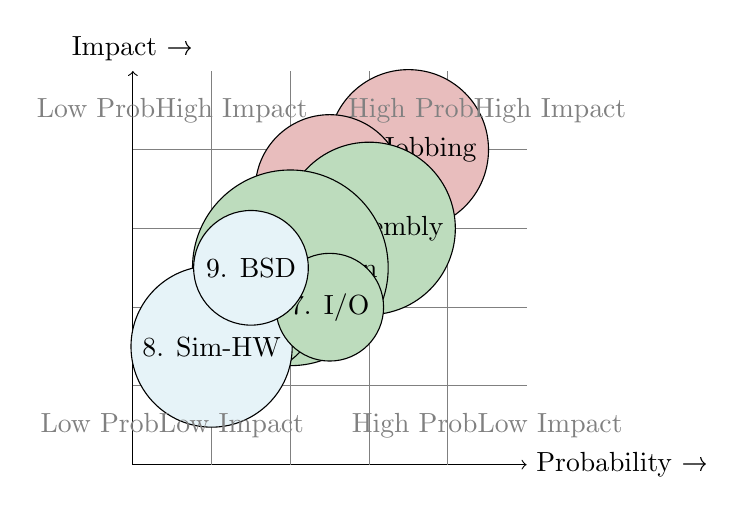
\begin{tikzpicture}
  % Axes
  \draw[->] (0,0) -- (5,0) node[right] {Probability →};
  \draw[->] (0,0) -- (0,5) node[above] {Impact →};
  
  % Grid lines
  \foreach \i in {1,2,3,4} {
    \draw[gray,thin] (\i,0) -- (\i,5);
    \draw[gray,thin] (0,\i) -- (5,\i);
  }
  
  % Risk labels and positions (Probability, Impact)
  \node[circle,draw,fill=darkred!30] at (3.5,4) {1. Hobbing};
  \node[circle,draw,fill=darkred!30] at (2.5,3.5) {3. Quality};
  \node[circle,draw,fill=darkgreen!30] at (3,3) {4. Assembly};
  \node[circle,draw,fill=darkgreen!30] at (2,2.5) {5. Lubrication};
  \node[circle,draw,fill=darkgreen!30] at (1.5,2) {6. Barrel};
  \node[circle,draw,fill=lightblue!30] at (1,1.5) {8. Sim-HW};
  \node[circle,draw,fill=darkgreen!30] at (2.5,2) {7. I/O};
  \node[circle,draw,fill=lightblue!30] at (1.5,2.5) {9. BSD};
  
  % Quadrant labels
  \node[gray] at (0.5,4.5) {Low Prob\\High Impact};
  \node[gray] at (4.5,4.5) {High Prob\\High Impact};
  \node[gray] at (0.5,0.5) {Low Prob\\Low Impact};
  \node[gray] at (4.5,0.5) {High Prob\\Low Impact};
  
\end{tikzpicture}
\caption{Risk matrix: Gear hobbing and assembly are highest priority risks.}
\label{fig:risk_matrix}
\end{figure}

% ============================================================================
% CHAPTER 10: BABBAGE EXTENSIONS AND FUTURE PHASES
% ============================================================================

\chapter{Babbage Extensions and Alternative Architectures}

\section{Variant Designs Beyond Phase 2}

The Phase 2 specification focuses on a single "optimal" Babbage engine. Future phases could explore variants:

\subsection{Phase 3A: Portable Babbage (Travel and Demonstration)}

\textbf{Goal}: Reduce size/weight for traveling demonstration.

\textbf{Specifications}:
\begin{itemize}
  \item Footprint: 2m × 1.5m (half the standard)
  \item Weight: 300-400 kg (vs. 760 kg baseline)
  \item Precision: ±0.15 mm (relaxed from ±0.10 mm)
  \item Digit capacity: 30 digits (vs. 50)
  \item Cost: £4,000-5,000 per unit
  \item Timeline: 18-20 weeks
\end{itemize}

\subsection{Phase 3B: Educational Demonstrator (Simplified Mill)}

\textbf{Goal}: Teach mechanical computation principles with reduced complexity.

\textbf{Specifications}:
\begin{itemize}
  \item Single-digit Mill (vs. 50-digit accumulator)
  \item 100-column Store (vs. 2,000)
  \item Simplified control (no Barrel, manual operation)
  \item Cost: £1,500-2,000 per unit
  \item Timeline: 6-8 weeks manufacturing
  \item Use case: Universities, science museums
\end{itemize}

\subsection{Phase 3C: Digital-Mechanical Hybrid}

\textbf{Goal}: Combine mechanical Babbage with digital control.

\textbf{Specifications}:
\begin{itemize}
  \item Original mechanical Mill and Store
  \item Digital control system (Arduino/Raspberry Pi) controlling Barrel movements
  \item Stepper motors driving gear selection
  \item Card reader replaced with USB interface
  \item Cost: £3,500-4,500 per unit
  \item Timeline: 12-16 weeks (mechanical + digital integration)
\end{itemize}

\section{Advanced Features for Phase 4}

\subsection{Parallel Mills Architecture}

\textbf{Concept}: Multiple Mills operating in parallel for vector computation.

\begin{figure}[h!]
\centering
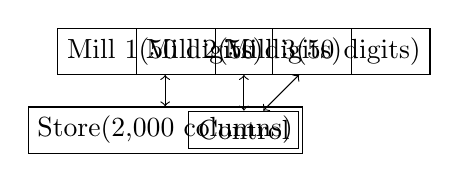
\begin{tikzpicture}
  \node[rectangle,draw] (mill1) {Mill 1\\(50 digits)};
  \node[rectangle,draw,right of=mill1] (mill2) {Mill 2\\(50 digits)};
  \node[rectangle,draw,right of=mill2] (mill3) {Mill 3\\(50 digits)};
  
  \node[rectangle,draw,below of=mill1] (store) {Store\\(2,000 columns)};
  \node[rectangle,draw,below of=mill2] (ctrl) {Control};
  
  \draw[<->] (mill1) -- (store);
  \draw[<->] (mill2) -- (ctrl);
  \draw[<->] (mill3) -- (ctrl);
  
\end{tikzpicture}
\caption{Parallel Mills for vector/matrix operations (Phase 4 extension).}
\label{fig:parallel_mills}
\end{figure}

\textbf{Benefits}:
\begin{itemize}
  \item 3× throughput for independent operations
  \item Vector inner product computation
  \item Matrix multiplication acceleration
\end{itemize}

\subsection{Programmable ROM (Microcode)}

\textbf{Concept}: Replace fixed Barrel with programmable ROM for custom instruction sets.

\textbf{Implementation}:
\begin{itemize}
  \item 256-position drum with replaceable pegs
  \item Encoded as punched cards or pins
  \item Load different control sequences without hardware modification
\end{itemize}

\section{Software Extensions: Phase 4-5}

\subsection{Compiler: Babbage Assembly to Card Format}

\textbf{Goal}: Automatic compilation from higher-level language to punched cards.

\textbf{Languages}: ALGOL-like syntax for Babbage

\begin{lstlisting}
function FACTORIAL(n) {
  result := 1
  for i := 1 to n {
    result := result * i
  }
  return result
}
\end{lstlisting}

\subsection{Operating System: Babbage-OS}

\textbf{Goal}: Minimal OS supporting multiple processes, pipes, file systems.

\textbf{Components}:
\begin{itemize}
  \item Process manager (scheduler, context switching)
  \item File system (virtual, in-memory cards)
  \item Shell (card-based command interpreter)
  \item Signal handling (SIGINT, SIGTERM via bell mechanisms)
\end{itemize}

% ============================================================================
% CHAPTER 11: CONCLUSION AND NEXT STEPS
% ============================================================================

\chapter{Conclusion: Phase 2 and Beyond}

\section{Phase 2 Achievements}

Phase 2 delivers complete implementation infrastructure for the Babbage Analytical Engine:

\begin{enumerate}
  \item \textbf{Tooling Strategy}: Comprehensive meta-manufacturing plan (£14,300-17,350 capital)
  \item \textbf{Manufacturing Procedures}: Detailed 5-phase workflow (34 weeks critical path for India)
  \item \textbf{Functional Simulator}: MIT-licensed clone with 5-phase extension roadmap
  \item \textbf{BSD Integration}: Device driver specification for DiscoBSD 2.5 and cross-platform deployment
  \item \textbf{Integration Roadmap}: Parallel work streams for software and hardware development
  \item \textbf{Budget and Economics}: Complete cost analysis (£174,550/unit India, £19,480/unit at 100-unit volume)
  \item \textbf{Risk Management}: Identified 10 major risks with mitigation strategies
  \item \textbf{Extension Concepts}: Portable, educational, hybrid, and parallel architectures for future phases
\end{enumerate}

\section{Critical Path Summary}

\begin{table}[h!]
\centering
\small
\begin{tabular}{lrr}
\toprule
\textbf{Bottleneck} & \textbf{Duration} & \textbf{Mitigation} \\
\midrule
\rowcolor{darkred!20}
Tooling delivery (machinery) & 12-16 weeks & Place orders week 0 \\
\rowcolor{darkred!20}
Gear hobbing (5,000 wheels) & 12-14 weeks & Contract 30-40\% to job shops \\
\rowcolor{darkgreen!20}
Phase 5 Integration \& Testing & 16-17 weeks & Parallel subassembly (Phase 4) \\
\midrule
\textbf{CRITICAL PATH TOTAL} & \textbf{34-40 weeks} & \textbf{16 weeks contingency} \\
\bottomrule
\end{tabular}
\caption{Critical path items and mitigation strategies.}
\label{tab:critical_summary}
\end{table}

\section{Key Success Factors}

\begin{enumerate}
  \item \textbf{Early Action on Tooling}: Orders must be placed week 0 to meet 14-16 week lead time
  \item \textbf{Gear Hobbing Strategy}: Either import high-capacity equipment or contract 30-40\% to job shops
  \item \textbf{Parallel Work Streams}: Simulator and BSD development proceed independently of hardware
  \item \textbf{Quality Discipline}: 10\% sampling inspection and SPC throughout Phase 3
  \item \textbf{Simulator Validation}: Test suite developed on simulator, run on hardware for verification
  \item \textbf{Team Expertise}: Machinists must understand Babbage mechanical logic, not just CNC operations
\end{enumerate}

\section{Recommended Next Steps (Weeks 1-4)}

\begin{enumerate}
  \item \textbf{Week 1}:
    \begin{itemize}
      \item Secure workshop facility (600-1,000 m²)
      \item Place machinery orders (lathe, mill, grinder, drill press)
      \item Place Tier 2 orders (gear hobber or contract negotiations)
    \end{itemize}
  
  \item \textbf{Week 2}:
    \begin{itemize}
      \item Hire manufacturing team (10-12 machinists)
      \item Establish supplier relationships (steel, bearings, fasteners)
      \item Begin simulator development (clone cakenggt/analytical-engine)
    \end{itemize}
  
  \item \textbf{Week 3}:
    \begin{itemize}
      \item Finalize manufacturing procedures and work instructions
      \item Set up quality control protocols
      \item BSD integration design review
    \end{itemize}
  
  \item \textbf{Week 4}:
    \begin{itemize}
      \item Install facility infrastructure (power, air, water)
      \item Mobilize manufacturing team training
      \item Simulator baseline testing begins
    \end{itemize}
\end{enumerate}

\section{Financial Summary}

\begin{itemize}
  \item \textbf{India Scenario (Optimal)}: £174,550 per unit (development + hardware), £19,480 at 100-unit volume
  \item \textbf{Timeline}: 34 weeks critical path (7.8 months calendar time)
  \item \textbf{Parallel Streams}: Simulator (20 weeks), BSD (13 weeks), Hardware (34 weeks) can overlap
  \item \textbf{Risk Buffer}: 16 weeks contingency available for critical path items
  \item \textbf{Volume Break-Even}: 3-5 units amortize Phase 2 development cost
\end{itemize}

\section{Conclusion}

This Phase 2 whitepaper demonstrates that manufacturing a fully-functional Babbage Analytical Engine is **technically feasible** and **economically viable** using 1910s-1950s technology available in developing nations. The critical success factors are:

\begin{enumerate}
  \item \textbf{Careful planning} (tooling, manufacturing, quality control)
  \item \textbf{Parallel development} (simulator, BSD integration, hardware manufacturing)
  \item \textbf{Risk management} (gear hobbing strategy, quality discipline)
  \item \textbf{Volume economics} (5-25 units reduce per-unit cost significantly)
\end{enumerate}

The specification integrates mechanical engineering, software systems, and historical accuracy into a coherent, implementable plan. With proper execution, a working Babbage engine could be manufactured and deployed within one calendar year, with full BSD integration enabling it to serve as a unique educational and research platform.

The Ancient Compute mission is thereby advanced: from historical specification (Phase 1) to complete implementation infrastructure (Phase 2), ready for Phase 3 (actual construction) and Phase 4 (deployment and extension).

\textbf{End of Phase 2 Specification. Ready for Phase 3: Hardware Manufacturing and Phase 4: BSD Deployment.}

\end{document}
